% !TeX root = Master.tex
\section{Results}
\label{sec:results}

We assess ranking fidelity according to Equation~\eqref{eq:ranking-preservation} across the iid, non-additive, group-correlated, and heteroskedastic ACIC 2017 error structures and all four N\&W DGPs at both sample sizes. Table~\ref{tab:rank-aggregation} reports Spearman rank correlations averaged over the 100 reference datasets in each setting, for individual simulators and rank aggregation, using all estimators and after excluding aligned estimators. For rank aggregation, exclusion removes aligned simulator votes. The \(\overline{|\Delta\Phi_s|}\) columns report mean absolute differences between simulator-induced and reference SACTEs. Figure~\ref{fig:promotion-shift} shows mean rank promotion and mean absolute rank shift separately for every setting. Table~\ref{tab:gcomp-selection} compares mean relative MSE regret from directly using the associated G-comp estimator with selecting an estimator from the full or family-excluded simulator ranking. Table~\ref{tab:distance-ranking} reports mean within-reference-dataset Pearson correlations between outcome-distribution distances and ranking fidelity across simulators. Appendix~\ref{app:complete-results} provides setting-specific MSEs (Table~\ref{tab:results_mse_all}), numerical ranking-fidelity and rank-movement results (Table~\ref{tab:results_rho_all}), and distributions of rank correlations (Figure~\ref{fig:acic_rho}).
\begin{table*}[!t]
\centering
\caption{Mean Spearman rank correlations and absolute estimand differences across 100 reference datasets per setting. All and Excl. use full and alignment-excluded rankings; aggregation follows Section~\ref{sec:benchmarking-procedure}. For each generator, bold, underlining, and gray shading mark the highest All correlation, highest Excl. correlation, and smallest mean absolute estimand difference, respectively. Counts: wins out of 12 settings, based on unrounded values.}
\label{tab:rank-aggregation}
{


\makebox[\textwidth][c]{%
\tablebox{%
\begin{tabular}{l@{\hspace{\tablegroupsep}}ccc@{\hspace{\tablegroupsep}}ccc@{\hspace{\tablegroupsep}}ccc@{\hspace{\tablegroupsep}}ccc@{\hspace{\tablegroupsep}}cc@{\hspace{\tablegroupsep}}cc}
\toprule
& \multicolumn{3}{c}{GB} & \multicolumn{3}{c}{NN} & \multicolumn{3}{c}{OLS2} & \multicolumn{3}{c}{RF} & \multicolumn{2}{c}{WGAN} & \multicolumn{2}{c}{Aggregated} \\
\cmidrule(lr){2-4}\cmidrule(lr){5-7}\cmidrule(lr){8-10}\cmidrule(lr){11-13}\cmidrule(lr){14-15}\cmidrule(lr){16-17}
Generator & All & Excl. & \(\overline{|\Delta\Phi_s|}\) & All & Excl. & \(\overline{|\Delta\Phi_s|}\) & All & Excl. & \(\overline{|\Delta\Phi_s|}\) & All & Excl. & \(\overline{|\Delta\Phi_s|}\) & All & \(\overline{|\Delta\Phi_s|}\) & All & Excl. \\
\midrule
ACIC IID & \textbf{0.946} & \underline{0.947} & \cellcolor{gray!20}0.095 & 0.814 & 0.856 & 0.140 & 0.128 & 0.682 & 0.939 & 0.804 & 0.881 & 0.213 & 0.068 & 1.379 & 0.919 & 0.934 \\
ACIC Non-additive & \textbf{0.945} & \underline{0.944} & \cellcolor{gray!20}0.116 & 0.848 & 0.885 & 0.193 & 0.092 & 0.614 & 1.228 & 0.684 & 0.803 & 0.352 & 0.082 & 1.852 & 0.899 & 0.928 \\
ACIC Group-correlated & \textbf{0.946} & \underline{0.951} & \cellcolor{gray!20}0.085 & 0.782 & 0.844 & 0.122 & 0.155 & 0.743 & 0.936 & 0.793 & 0.880 & 0.206 & 0.042 & 1.400 & 0.916 & 0.932 \\
ACIC Heteroskedastic & \textbf{0.942} & \underline{0.943} & \cellcolor{gray!20}0.089 & 0.798 & 0.848 & 0.145 & 0.141 & 0.707 & 0.941 & 0.805 & 0.883 & 0.207 & 0.061 & 1.366 & 0.912 & 0.929 \\
N\&W A, $n=1000$ & \textbf{0.504} & 0.384 & \cellcolor{gray!20}0.077 & 0.134 & 0.207 & 0.175 & 0.474 & \underline{0.495} & 0.099 & -0.046 & 0.027 & 0.137 & 0.245 & 0.448 & 0.317 & 0.305 \\
N\&W A, $n=4302$ & \textbf{0.367} & \underline{0.569} & \cellcolor{gray!20}0.046 & 0.277 & 0.193 & 0.091 & 0.104 & 0.116 & 0.087 & -0.344 & -0.230 & 0.087 & 0.321 & 0.203 & 0.127 & 0.186 \\
N\&W B, $n=1000$ & 0.543 & 0.706 & 0.079 & 0.929 & 0.920 & 0.057 & \textbf{0.936} & \underline{0.933} & \cellcolor{gray!20}0.055 & 0.068 & 0.180 & 0.231 & 0.628 & 0.370 & 0.787 & 0.810 \\
N\&W B, $n=4302$ & 0.316 & 0.512 & 0.039 & \textbf{0.899} & 0.906 & 0.033 & 0.854 & \underline{0.913} & \cellcolor{gray!20}0.030 & -0.087 & -0.073 & 0.110 & 0.570 & 0.106 & 0.733 & 0.740 \\
N\&W C, $n=1000$ & 0.328 & 0.560 & 0.196 & 0.949 & 0.954 & 0.074 & \textbf{0.978} & \underline{0.975} & \cellcolor{gray!20}0.056 & -0.112 & 0.119 & 0.585 & 0.466 & 0.546 & 0.760 & 0.774 \\
N\&W C, $n=4302$ & -0.119 & 0.029 & 0.095 & 0.805 & 0.857 & 0.039 & \textbf{0.957} & \underline{0.946} & \cellcolor{gray!20}0.029 & -0.634 & -0.528 & 0.376 & 0.322 & 0.210 & 0.494 & 0.406 \\
N\&W D, $n=1000$ & 0.434 & 0.421 & 0.089 & \textbf{0.840} & \underline{0.808} & \cellcolor{gray!20}0.069 & 0.700 & 0.729 & 0.079 & 0.395 & 0.435 & 0.102 & 0.511 & 0.421 & 0.778 & 0.753 \\
N\&W D, $n=4302$ & 0.455 & 0.605 & 0.040 & \textbf{0.900} & \underline{0.911} & \cellcolor{gray!20}0.040 & 0.524 & 0.827 & 0.059 & 0.324 & 0.477 & 0.044 & 0.598 & 0.119 & 0.807 & 0.839 \\
% BEGIN WIN COUNTS
\midrule
Winner count & 6/12 & 5/12 & 6/12 & 3/12 & 2/12 & 2/12 & 3/12 & 5/12 & 4/12 & 0/12 & 0/12 & 0/12 & 0/12 & 0/12 & 0/12 & 0/12 \\
% END WIN COUNTS
\bottomrule
\end{tabular}%
}
}
}
\end{table*}

\begin{figure*}[!t]
\centering
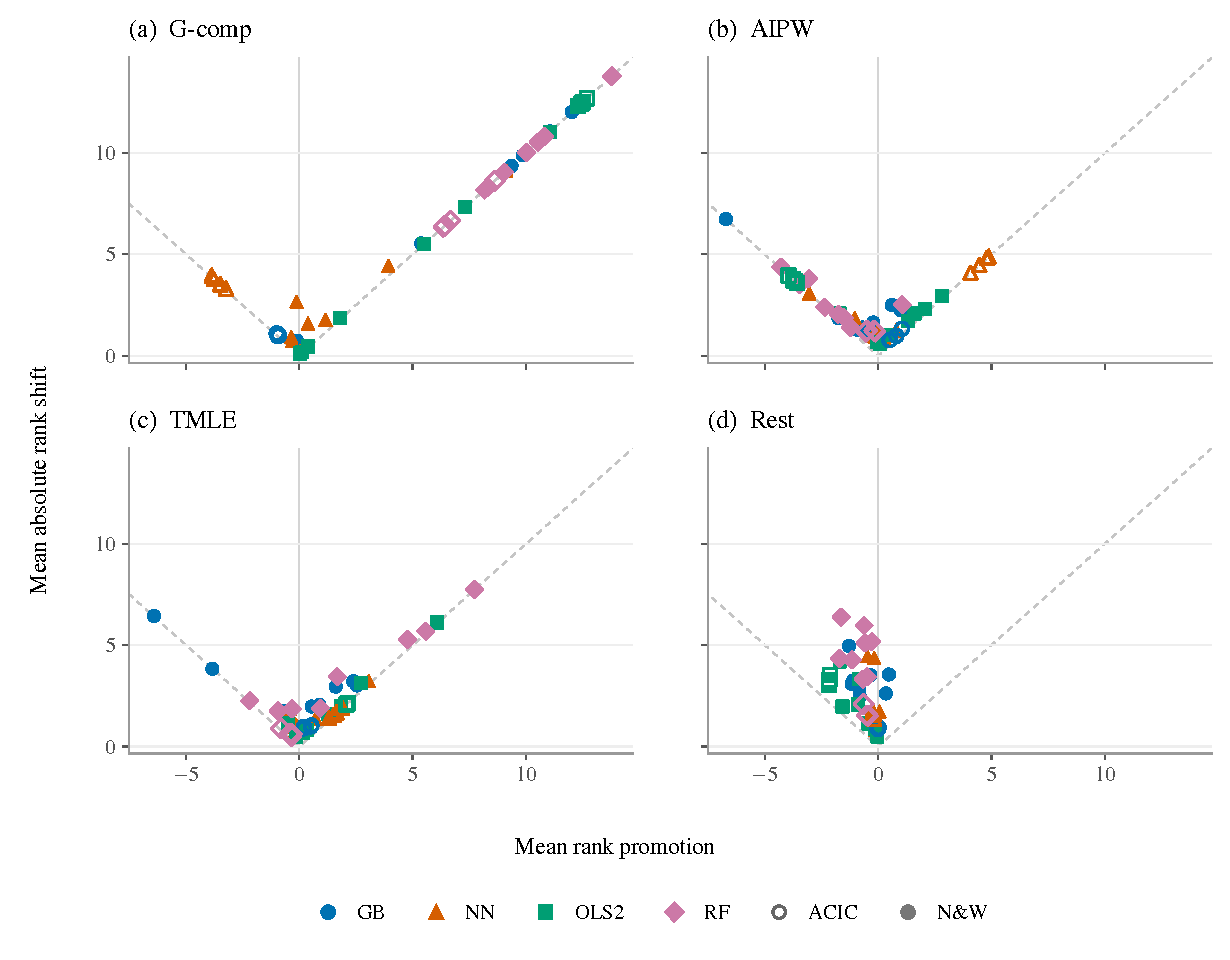
\includegraphics[width=0.75\textwidth]{figures/promotion_shift/promotion_shift.pdf}
\caption{Mean rank promotion and mean absolute rank shift for the associated G-comp, aligned AIPW, aligned TMLE, and non-aligned estimators (Rest; OLS1 is considered aligned with OLS2). Each point summarizes 100 reference datasets for one simulator and setting: open markers denote the four ACIC error structures; filled markers denote the eight N\&W DGP--sample-size settings. Colors and marker shapes identify simulators. Rest averages over non-aligned estimators; because promotions sum to zero, net aligned promotion implies net Rest demotion. Positive promotion indicates a higher rank under the simulator. The dashed boundary is $y=|x|$; points above it indicate rank movement in both directions across reference datasets (and, for Rest, estimators).}
\label{fig:promotion-shift}
\end{figure*}

\subsection{Ranking fidelity}

The fitted simulators can attain high ranking fidelity, but no single simulator performs best across all generators.

Table~\ref{tab:rank-aggregation} shows that, for ACIC, GB gives the highest mean rank correlation in each of the four error settings (0.942--0.946). NN (0.782--0.848) and RF (0.684--0.805) also attain relatively high correlations, although their ordering differs across error structures. RF has similar ranking fidelity under iid, group-correlated, and heteroskedastic errors (0.793--0.805), but its mean rank correlation falls to 0.684 under non-additive errors. GB remains stable, while NN has its highest mean rank correlation in the non-additive setting (0.848). OLS2 and WGAN have low ranking fidelity throughout (0.092--0.155 and 0.042--0.082, respectively). Overall, error structure appears to have a limited effect on ranking fidelity, with the clearest exception being RF under non-additive errors. Averaging the five simulator-specific rankings gives mean rank correlations of 0.899--0.919, below GB in every setting but above the other individual simulators. The aggregate mean rank correlation is lowest under non-additive errors.

The WGAN's low ranking fidelity in ACIC occurred despite diagnostic comparisons (not shown) similar to those presented by \authorcite{atheyUsingWassersteinGenerative2024}, in which the generated outcome distributions appeared reasonably similar to the observed ones. These checks therefore did not establish ranking fidelity.

The N\&W designs show stronger variation across settings and sample sizes (Table~\ref{tab:rank-aggregation}). GB has the highest mean rank correlation in A at both sample sizes (0.504 and 0.367), while OLS2 and NN perform best in B and C: OLS2 reaches 0.978 and 0.957 in C, and NN leads in B at \(n=4302\) (0.899). NN also leads in D, improving from 0.840 to 0.900 as the sample size increases. Larger samples do not uniformly improve ranking fidelity, however: in C, GB's mean rank correlation falls from 0.328 to -0.119 and RF's from -0.112 to -0.634. Rank aggregation gives mean rank correlations of 0.127--0.807 and remains below the best individual simulator in each setting. In C at \(n=4302\), for example, the aggregate mean rank correlation is 0.494 compared with 0.957 for OLS2. Averaged over all eight settings, NN has the highest mean rank correlation (0.717), followed by OLS2 (0.691), WGAN (0.458), GB (0.354), and RF (-0.055) (Table~\ref{tab:results_rho_all}).

\subsection{Model alignment}

Figure~\ref{fig:promotion-shift} shows that alignment affects estimator classes differently. G-comp exhibits the strongest upward rank promotion, whereas TMLE shows smaller and more variable promotion. AIPW promotions are generally centered near zero, with movement in both directions rather than a systematic upward shift. NN in ACIC is an exception, with aligned AIPW promoted by approximately four to five positions. Small mean promotion can also conceal movement in both directions, as indicated by points above the dashed boundary. Thus, sharing the simulator's outcome learner does not uniformly benefit all three estimator classes.

The largest G-comp promotions occur for OLS2 in ACIC, GB in N\&W, and RF in both design families. Table~\ref{tab:rank-aggregation} supports the importance of these aligned estimators for ranking disagreement: excluding them raises OLS2's ACIC rank correlations from 0.092--0.155 to 0.614--0.743 and RF's from 0.684--0.805 to 0.803--0.883. For GB in N\&W C at \(n=1000\), the correlation increases from 0.328 to 0.560. RF also improves after exclusion in every N\&W setting, although its correlation remains negative in several settings, including C at \(n=4302\) (-0.634 to -0.528). Alignment therefore explains part, but not all, of the ranking disagreement. These pronounced G-comp promotions coincide with poor target-benchmark performance of the associated G-comp estimators (Appendix Table~\ref{tab:results_mse_all}). In contrast, GB in ACIC shows little rank movement, and exclusion barely changes its correlations (0.942--0.946 versus 0.943--0.951). However, estimators already near the top of the target ranking have little room for promotion; an estimator ranked first can only remain first or be demoted. Small rank movements therefore do not rule out an accuracy gain under an aligned simulator. Still, comparing MSEs in Appendix Table~\ref{tab:results_mse_all} suggests that this is not the case for GB in ACIC.

Excluding aligned votes also changes rank aggregation (Table~\ref{tab:rank-aggregation}). In ACIC, correlations increase from 0.899--0.919 to 0.928--0.934. The N\&W results are mixed: exclusion improves aggregation in some settings, but lowers it in C at \(n=4302\) and D at \(n=1000\).

\subsection{Estimand fidelity and ranking fidelity}

Table~\ref{tab:rank-aggregation} reports mean absolute estimand differences alongside rank correlations; smaller differences indicate higher \emph{estimand fidelity}. Across the settings studied, high ranking fidelity is generally accompanied by high estimand fidelity. GB has the smallest mean absolute estimand difference in every ACIC setting (0.085--0.116), while OLS2 combines the smallest differences (0.029--0.056) with high ranking fidelity in N\&W B and C.

In some settings, however, high estimand fidelity is not accompanied by high ranking fidelity. Table~\ref{tab:rank-aggregation} shows that simulators can have similar mean absolute estimand differences but substantially different rank correlations. In N\&W B at \(n=4302\), GB has an estimand difference of 0.039, close to those of OLS2 (0.030) and NN (0.033), but a much lower mean rank correlation (0.316 versus 0.854 and 0.899). In D at the same sample size, GB and NN both have differences of approximately 0.040, yet mean rank correlations of 0.455 and 0.900. Excluding aligned estimators does not remove these contrasts: GB reaches only 0.512 in B and 0.605 in D, compared with NN's 0.906 and 0.911. The limitation is also evident for RF in A and D at \(n=4302\): relatively small differences (0.087 and 0.044) accompany mean rank correlations of -0.344 and 0.324, which remain -0.230 and 0.477 after exclusion.

\subsection{Estimator-selection regret}
\begin{table*}[!t]
\centering
\caption{Mean relative MSE regret (\%) across the 100 reference datasets in each setting. Within each dataset, regret is the percentage excess target-benchmark MSE over the smallest target MSE among all 15 estimators; these percentages are then averaged over the 100 reference datasets. So 0 means matching the target-best MSE, and 100 means twice that MSE. G-comp uses the associated G-computation estimator directly. All and Excl. use the estimator minimizing simulator MSE among all estimators or among non-aligned estimators, respectively. Bold marks the lowest value within each simulator--setting triplet, including ties. WGAN is omitted because it has no associated G-comp in the candidate set.}
\label{tab:gcomp-selection}
{
\tablebox{%
\begin{tabular}{l*{12}{r}}
\toprule
Generator & \multicolumn{3}{c}{GB} & \multicolumn{3}{c}{NN} & \multicolumn{3}{c}{OLS2} & \multicolumn{3}{c}{RF} \\
\cmidrule(lr){2-4}\cmidrule(lr){5-7}\cmidrule(lr){8-10}\cmidrule(lr){11-13}
 & G-comp & All & Excl. & G-comp & All & Excl. & G-comp & All & Excl. & G-comp & All & Excl. \\
\midrule
ACIC IID & \textbf{1.6} & 17.6 & 31.1 & 202.1 & 148.0 & \textbf{63.3} & 6647.4 & 6678.3 & \textbf{187.2} & 381.9 & 178.2 & \textbf{62.3} \\
ACIC Non-additive & \textbf{0.0} & 27.6 & 46.7 & 224.9 & 135.9 & \textbf{57.3} & 6944.1 & 7001.6 & \textbf{203.4} & 629.0 & 550.5 & \textbf{250.6} \\
ACIC Group-correlated & \textbf{0.9} & 18.5 & 30.6 & 97.9 & 153.9 & \textbf{81.1} & 7931.3 & 7962.7 & \textbf{93.3} & 446.3 & 198.4 & \textbf{71.3} \\
ACIC Heteroskedastic & \textbf{1.1} & 20.8 & 30.7 & 162.9 & 149.2 & \textbf{62.8} & 7013.1 & 7023.5 & \textbf{155.2} & 382.9 & 167.1 & \textbf{64.2} \\
\addlinespace[\tablepanelgap]
N\&W A, $n=1000$ & \textbf{1.3} & 26.8 & 44.7 & 216.9 & 168.2 & \textbf{156.0} & 47.2 & 45.8 & \textbf{3.4} & 175.7 & \textbf{131.9} & \textbf{131.9} \\
N\&W A, $n=4302$ & 70.9 & 60.8 & \textbf{28.9} & 508.2 & \textbf{137.9} & 138.0 & 351.2 & 351.2 & \textbf{69.9} & 421.8 & 325.2 & \textbf{312.9} \\
N\&W B, $n=1000$ & 115.5 & 79.3 & \textbf{28.4} & 9.4 & \textbf{3.6} & 4.1 & \textbf{2.6} & 2.9 & 10.7 & 1720.1 & 250.2 & \textbf{113.9} \\
N\&W B, $n=4302$ & 117.7 & 74.2 & \textbf{18.1} & 17.4 & \textbf{1.9} & 2.0 & \textbf{3.5} & \textbf{3.5} & 4.3 & 1698.6 & 160.5 & \textbf{117.5} \\
N\&W C, $n=1000$ & 779.1 & 727.8 & \textbf{227.5} & 47.3 & 15.6 & \textbf{8.2} & 0.6 & \textbf{0.4} & 43.6 & 6792.2 & 5590.6 & \textbf{779.1} \\
N\&W C, $n=4302$ & 812.5 & 649.9 & \textbf{460.3} & 39.9 & 23.1 & \textbf{15.3} & \textbf{0.1} & \textbf{0.1} & 33.5 & 12797.6 & 10333.9 & \textbf{1054.7} \\
N\&W D, $n=1000$ & \textbf{69.1} & 87.8 & 95.7 & \textbf{3.7} & 16.9 & 27.5 & 53.7 & 53.7 & \textbf{15.4} & 99.6 & 99.8 & \textbf{81.3} \\
N\&W D, $n=4302$ & 65.2 & 50.7 & \textbf{45.8} & 15.7 & \textbf{3.1} & 5.0 & 189.8 & 189.8 & \textbf{1.5} & 116.4 & 65.2 & \textbf{60.6} \\
% BEGIN WIN COUNTS
\midrule
Winner count & 6/12 & 0/12 & 6/12 & 1/12 & 4/12 & 7/12 & 1/12 & 3/12 & 8/12 & 0/12 & 1/12 & 12/12 \\
% END WIN COUNTS
\bottomrule
\end{tabular}%
}
}
\end{table*}


Table~\ref{tab:gcomp-selection} reports the mean relative MSE regret defined in Equation~\eqref{eq:relative-mse-regret}. It shows that simulator-based selection can be valuable even when ranking fidelity is poor, particularly after excluding aligned estimators. For example, under the OLS2 simulator in ACIC, direct G-comp and All-based selection both have mean relative MSE regret above 6600\%, whereas Excl.-based selection has the lowest regret of the three choices in every error setting (93.3--203.4\%). The same pattern appears for RF in N\&W C at \(n=4302\): regret falls from 12797.6\% for RF G-comp and 10333.9\% for All-based selection to 1054.7\% after exclusion. Although the remaining loss is substantial, selecting a non-aligned estimator is much preferable to directly using the poorly performing associated G-comp in these settings.

This benefit is not confined to the simulators with the lowest ranking fidelity. NN has comparatively high ranking fidelity in ACIC, yet Excl.-based selection gives the lowest mean regret in every error setting: 57.3--81.1\%, compared with 97.9--224.9\% for NN G-comp and 135.9--153.9\% for All-based selection. Thus, selection among non-aligned estimators using a reasonably faithful simulator can outperform direct G-comp based on its associated conditional-mean learner.

When the associated outcome model performs well, directly using G-comp can instead be preferable. GB G-comp has mean regret below 1.7\% throughout ACIC, compared with 17.6--27.6\% for All-based selection and 30.6--46.7\% after exclusion. OLS2 in N\&W B and C also favors direct G-comp or gives nearly indistinguishable results with All-based selection: at \(n=4302\), both choices have mean regret of 3.5\% in B and 0.1\% in C, while Excl.-based selection gives 4.3\% and 33.5\%, respectively. In these examples, the penalty for following the ranking rather than using a well-performing G-comp is much smaller than the loss from directly using the poor OLS2 or RF G-comp estimators instead of Excl.-based selection in the earlier comparisons.

\subsection{Outcome-distribution distances}

\begin{table*}[!t]
\centering
\caption{Mean within-reference-dataset Pearson correlations between outcome-distribution distance and Spearman ranking fidelity. The main panels compare all five simulators; sensitivity panels remove WGAN in ACIC and RF in N\&W, leaving four. Each correlation compares these simulators on the same reference dataset; coefficients are then averaged over the 100 reference datasets. All and Excl. aligned use ranking fidelity before and after excluding estimators aligned with each simulator, respectively. Negative values indicate that simulators with smaller distances tend to have higher ranking fidelity. Bold marks the most negative mean correlation within each setting and estimator panel, including ties based on unrounded means. Superscripts \(\dagger\), \(\ddagger\), and \(\S\) indicate negative correlations in at least 90\%, 95\%, and 99\% of reference datasets, respectively (do not confuse with significance levels). }
\label{tab:distance-ranking}
{
\makebox[\textwidth][c]{\begin{tabular}{lrrrr@{\hspace{\tablegroupsep}}rrrrrrrr@{\hspace{\tablegroupsep}}r}
\toprule
& \multicolumn{4}{c}{ACIC 2017} & \multicolumn{8}{c}{N\&W} & Winner count \\
\cmidrule(lr){2-5}\cmidrule(lr){6-13}\cmidrule(lr){14-14}
Distance & IID & \shortstack{Non-\\additive} & \shortstack{Group-\\correlated} & \shortstack{Hetero-\\skedastic} & \shortstack{A\\$n=1000$} & \shortstack{A\\$n=4302$} & \shortstack{B\\$n=1000$} & \shortstack{B\\$n=4302$} & \shortstack{C\\$n=1000$} & \shortstack{C\\$n=4302$} & \shortstack{D\\$n=1000$} & \shortstack{D\\$n=4302$} & Total \\
\midrule
\multicolumn{14}{l}{\textit{All estimators}} \\
$W_1$ & -0.049 & -0.402 & -0.119 & -0.071 & 0.029 & \textbf{-0.098} & \textbf{-0.159} & \textbf{-0.392} & \textbf{-0.261} & \textbf{-0.420} & \textbf{-0.344} & \textbf{-0.389} & 7/12 \\
KS & \textbf{-0.351} & \textbf{-0.539}\textsuperscript{\(\dagger\)} & \textbf{-0.422} & \textbf{-0.377} & 0.015 & 0.116 & -0.009 & -0.041 & -0.027 & -0.042 & -0.192 & -0.146 & 4/12 \\
Energy & -0.179 & -0.529 & -0.254 & -0.209 & \textbf{0.015} & -0.004 & -0.097 & -0.247 & -0.194 & -0.313 & -0.276 & -0.288 & 1/12 \\
\addlinespace[\tablepanelgap]
\multicolumn{14}{l}{\textit{Excl. aligned}} \\
$W_1$ & -0.329 & -0.569 & -0.413 & -0.365 & \textbf{-0.058} & \textbf{0.001} & \textbf{-0.186} & \textbf{-0.424}\textsuperscript{\(\dagger\)} & \textbf{-0.337} & \textbf{-0.452} & \textbf{-0.383} & \textbf{-0.539} & 8/12 \\
KS & \textbf{-0.662}\textsuperscript{\(\dagger\)} & \textbf{-0.706}\textsuperscript{\(\dagger\)} & \textbf{-0.736}\textsuperscript{\(\dagger\)} & \textbf{-0.706}\textsuperscript{\(\ddagger\)} & -0.025 & 0.071 & -0.078 & -0.110 & -0.142 & -0.085 & -0.221 & -0.265 & 4/12 \\
Energy & -0.482 & -0.680 & -0.566\textsuperscript{\(\dagger\)} & -0.527 & -0.046 & 0.034 & -0.142 & -0.300 & -0.287 & -0.351 & -0.316 & -0.451 & 0/12 \\
\addlinespace[\tablepanelgap]
\multicolumn{14}{l}{\textit{All estimators; WGAN / RF removed}} \\
$W_1$ & 0.386 & -0.254 & 0.376 & 0.384 & -0.051 & 0.366 & \textbf{-0.602}\textsuperscript{\(\ddagger\)} & \textbf{-0.488} & \textbf{-0.620}\textsuperscript{\(\dagger\)} & \textbf{-0.475} & \textbf{-0.453} & \textbf{-0.329} & 6/12 \\
KS & \textbf{0.334} & -0.457\textsuperscript{\(\ddagger\)} & \textbf{0.315} & \textbf{0.322} & \textbf{-0.174} & \textbf{0.253} & -0.455 & -0.220 & -0.392 & -0.136 & -0.303 & -0.192 & 5/12 \\
Energy & 0.379 & \textbf{-0.585}\textsuperscript{\(\ddagger\)} & 0.366 & 0.372 & -0.115 & 0.325 & -0.540\textsuperscript{\(\dagger\)} & -0.367 & -0.568\textsuperscript{\(\dagger\)} & -0.358 & -0.390 & -0.269 & 1/12 \\
\addlinespace[\tablepanelgap]
\multicolumn{14}{l}{\textit{Excl. aligned; WGAN / RF removed}} \\
$W_1$ & 0.342 & -0.302 & 0.281 & 0.331 & -0.153 & 0.395 & \textbf{-0.679}\textsuperscript{\(\ddagger\)} & \textbf{-0.618}\textsuperscript{\(\ddagger\)} & \textbf{-0.717}\textsuperscript{\(\ddagger\)} & \textbf{-0.530}\textsuperscript{\(\dagger\)} & \textbf{-0.478} & \textbf{-0.522} & 6/12 \\
KS & \textbf{0.256} & -0.494\textsuperscript{\(\dagger\)} & \textbf{0.177} & \textbf{0.230} & \textbf{-0.198} & \textbf{0.142} & -0.600\textsuperscript{\(\dagger\)} & -0.407 & -0.528 & -0.204 & -0.319 & -0.316 & 5/12 \\
Energy & 0.323 & \textbf{-0.585}\textsuperscript{\(\ddagger\)} & 0.254 & 0.305 & -0.177 & 0.291 & -0.649\textsuperscript{\(\dagger\)} & -0.529\textsuperscript{\(\dagger\)} & -0.684\textsuperscript{\(\ddagger\)} & -0.419 & -0.414 & -0.457 & 1/12 \\
\bottomrule
\end{tabular}}
}
\end{table*}


For each reference dataset, we compute the Pearson correlation across the five simulators between outcome-distribution distance and ranking fidelity, then average these correlations over the 100 reference datasets in each setting. Negative correlations indicate that simulators whose generated outcomes are closer to the observed outcomes tend to give more faithful rankings on the same reference dataset.

With all five simulators, Table~\ref{tab:distance-ranking} shows predominantly negative mean correlations, generally stronger after excluding aligned estimators. KS has the most negative mean correlation in every ACIC setting, both before and after exclusion. In N\&W, Wasserstein distance has the most negative mean correlation in seven of eight settings before exclusion and all eight afterward. The N\&W associations are clearest in B--D, while those in A are near zero or mixed in sign.

These averages conceal substantial variation across reference datasets. In the five-simulator analysis, only one comparison using all estimators and six after excluding aligned estimators have negative correlations in at least 90\% of reference datasets. The highest proportion is 95\%, attained by KS in the ACIC heteroskedastic setting after exclusion.

Furthermore, each correlation uses only five simulators and is therefore sensitive to individual simulators with extreme distances or ranking fidelity. Table~\ref{tab:distance-ranking} also reports sensitivity checks removing the simulator with the lowest ranking fidelity in each design family. Removing WGAN in ACIC reversed the mean correlations from negative to positive for all three distances in every setting except non-additive errors, both before and after excluding aligned estimators. Removing RF in N\&W, by contrast, generally strengthened the negative associations in B--D: all three distances retained negative mean correlations at both sample sizes, before and after exclusion. In A, the correlations remained inconsistent, becoming negative at \(n=1000\) and positive at \(n=4302\) for all three distances and both estimator sets.
